\newsection
\section{Технический проект}
\subsection{Общая характеристика организации решения задачи}

разработать веб-сайт, который должен способствовать продвижению компании на рынке.
Веб-сайт-это набор взаимосвязанных электронных страниц, которые сгруппированы в разделы, содержащие текстовую, графическую и мультимедийную информацию.Сайт находится в Интернете по определенному адресу . Каждая страница веб-сайта представляет собой текстовый документ, написанный на языке программирования (HTML, CSS, JavaScript и т. Д.).

\subsection{Обоснование выбора технологии проектирования}

Сегодня информационный рынок, предоставляющий программные решения в выбранной области, предлагает множество продуктов, которые позволяют достичь поставленной цели - разработки веб-сайта.

\subsubsection{Описание используемых технологий и языков программирования}

В процессе разработки веб-сайта используются программные средства и языки программирования. Каждый программный инструмент и каждый язык программирования используются для решения ряда задач, для которых они необходимы.

\subsubsection{Язык программирования HTML}

HTML (Hypertext Markup Language) - одна из самых фундаментальных технологий, используемых в веб-программировании. HTML используется для определения структуры и содержания веб-страницы, т.е. элементов,
составляющих веб-страницу, и их иерархической организации.
В дополнение к HTML существуют и другие технологии, такие как CSS
(каскадные таблицы стилей), которые позволяют определять стили и визуальный формат веб-страницы. Существует также JavaScript, третья фундаментальная технология, которая используется для придания страницам интерактивности и динамичности.
HTML был разработан в начале 1990-х годов и с течением времени развивался, включая новые функции и возможности. Совет Всемирной паутины
(W3C) является организацией, ответственной за разработку и поддержание
стандартов HTML
авыки, необходимые для изучения HTML, включают понимание тегов, базовой структуры веб-страницы, атрибутов, ссылок, форм, а также использование изображений и видео.
В целом, HTML - это важный язык разметки, используемый для разработки современных веб-страниц и являющийся фундаментальным компонентом веб-программирования.
Использование HTML на веб-странице в клинической лаборатории - обычное дело, поскольку HTML - это язык, используемый для создания веб- страниц. HTML, что расшифровывается как HyperText Markup Language, - это
язык разметки, который используется для создания структурированного веб-контента. Использование HTML позволяет легко создать организованную и
удобную веб-страницу для пациентов.
HTML-теги позволяют организовать содержимое веб-страницы в различные разделы, такие как заголовки, абзацы, таблицы, изображения, формы
и ссылки. Клинические лаборатории могут использовать эти теги, чтобы сделать свою информацию легко читаемой и доступной для пациентов.
Дизайн и внешний вид веб-сайта также должны соответствовать клиническому имиджу лаборатории. Поэтому используйте соответствующую цветовую схему и убедитесь, что содержание представлено профессионально и
понятно.
Использование HTML на сайте клинической лаборатории является
очень распространенным, поскольку именно с его помощью создается структура и содержание сайта.


\subsubsection{Язык программирования PHP}

РНР изобретен Расмусом Лердорфом в конце 1994 года. Первая версия выпущена в 1995 году под именем «Инструментарий Персональных Домашних Страниц», затем она была переработана и названа PHP/FI Version 2 (FI -- модуль обработки данных для форм). Также была добавлена поддержка баз данных mSQL. С этого момента в разработке стали принимать участие добровольцы.

Статистика используемости РНР приблизительна, но, согласно исследованию, проведенному Netcraft, в начале 2001 года РНР использовался на более чем 5 300 000 сайтах по всему миру. Для сравнения: в это время число IIS серверов было примерно таким же (5 млн). Разработка интерпретатора РНР приняла форму организованного командного процесса, ядро интерпретатора разрабатывает компания Zend.com. При этом РНР распространяется свободно: его последнюю версию можно загрузить с сайта PHP.net. Модули РНР поставляются в комплекте с сервером Apache, в комплектах систем Linux.

Изначально аббревиатура РНР означала Preprocessor of Home Pages -- препроцессор домашних страниц. Это язык внедряемых в HTML-страницы сценариев, исполняемых на сервере. По большей части его синтаксис заимствован из таких языков, как С, Perl, Java, и при этом добавлена масса возможностей, которых этим языкам недостает. Проще говоря, синтаксис РНР -- это разумная альтернатива и строгости С, и «беспредельности» Perl.


\subsubsection{Язык программирования JavaScript}

JavaScript - это язык программирования, который разработчики используют для создания интерактивных веб-страниц. Функции JavaScript, от обновления каналов социальных сетей до отображения анимации и интерактивных карт, могут улучшить взаимодействие пользователя с веб-сайтом. Как язык сценариев на стороне сервера, это одна из основных технологий Всемирной Паутины. Например, при просмотре веб-страниц в любое время, когда вы видите карусель изображений, раскрывающееся меню “щелкнуть, чтобы отобразить” или динамическое изменение цветовых элементов на веб-странице, вы будете видеть эффекты JavaScript.

Microsoft SQL Server — это система управления реляционными базами данных (RDBMS), которая поддерживает широкий спектр приложений для обработки транзакций, бизнес-аналитики и аналитики в корпоративных вычислительных средах. Microsoft SQL Server — одна из трех ведущих технологий баз данных на рынке, наряду с Oracle Database и IBM DB2.

Как и другие программы RDBMS, Microsoft SQL Server основан на SQL, стандартизированном языке программирования, который администраторы баз данных (DBA) и другие ИТ-специалисты используют для управления базами данных и запросов к содержащимся в них данным. SQL Server связан с Transact-SQL (T-SQL), реализацией SQL от Microsoft, которая добавляет набор проприетарных программных расширений к стандартному языку.

Внутри архитектуры SQL Server: как работает SQL Server Подобно другим технологиям СУБД, SQL Server в основном построен на базе табличной структуры, основанной на строках, которая связывает связанные элементы данных в разных таблицах друг с другом, избегая необходимости избыточного хранения данных в нескольких местах в таблице, базе данных. Реляционная модель также обеспечивает ссылочную целостность и другие ограничения целостности для поддержания точности данных. Эти проверки являются частью более широкой приверженности принципам атомарности, непротиворечивости, изоляции и устойчивости, известным под общим названием свойства ACID, и предназначены для обеспечения надежной обработки транзакций базы данных.

\subsubsection{Язык программирования C\#}

Это объектно-ориентированный язык программирования, разработанный Microsoft и предназначенный для создания различных приложений, работающих на платформе .NET Framework. Это простой, мощный и типобезопасный язык. Множество нововведений в C\# позволяют быстро разрабатывать приложения, сохраняя при этом выразительность и элегантность языков в стиле C.

Это отрасль компьютерных наук, которая использует в качестве собственного названия объекты и их взаимодействия для разработки приложений и компьютерных программ. Следует отметить, что программный объект — это объект, который сочетает в себе состояние (это данные объекта), поведение или метод (те, которые определяют, какие операции может выполнять объект) и идентичность (это отличающий фактор от других объектов).

C\# рассматривается как эволюция и потребность в определенных обстоятельствах. Эволюция из-за языков-предшественников, которыми являются C и C++, и необходимости в то время, когда у компании были проблемы с компанией, создавшей язык Java. Именно по этой причине C Sharp представляет положительные качества C++, Java и Visual Basic и улучшает их, предоставляя сильный и обновленный язык для современности.

Синтаксис унаследован от C и C++ и использует объектную модель платформы .NET, очень похожую на модель Java, хотя и включает усовершенствования других языков .NET. Любопытно, что название этого языка было навеяно музыкальной гаммой. В нем буква до эквивалентна музыкальной ноте до, а символ \# означает выдержанный, что указывает на то, что она на полтона выше. Таким образом, C\# предполагает, что он превосходит C и C+

\subsubsection{Язык программирования CSS}

Каскадные таблицы стилей (CSS) — это язык таблиц стилей, используемый для описания представления документа, написанного на языке разметки, таком как HTML или XML (включая диалекты XML, такие как SVG, MathML или XHTML). CSS является краеугольным камнем технологии World Wide Web, наряду с HTML и JavaScript.

CSS предназначен для разделения содержимого и представления, включая макет, цвета и шрифты.[3] Такое разделение может улучшить доступность контента; обеспечить большую гибкость и контроль в спецификации характеристик презентации; разрешить нескольким веб-страницам совместное форматирование, указав соответствующий CSS в отдельном файле .css, что снижает сложность и повторяемость структурного содержимого; и включите кэширование файла .css, чтобы повысить скорость загрузки страницы между страницами, которые совместно используют файл и его форматирование.

Разделение форматирования и содержимого также делает возможным представление одной и той же страницы разметки в разных стилях для разных методов рендеринга, например, на экране, в печати, голосом (через речевой браузер или программу чтения с экрана) и на основе Брайля. тактильные устройства. В CSS также есть правила для альтернативного форматирования, если доступ к содержимому осуществляется с мобильного устройства.

Каскадирование имен исходит из указанной схемы приоритетов, чтобы определить, какое правило стиля применяется, если более одного правила соответствует определенному элементу. Эта каскадная схема приоритетов предсказуема.

Спецификации CSS поддерживаются Консорциумом World Wide Web (W3C). Тип интернет-медиа (тип MIME) text/css зарегистрирован для использования с CSS в соответствии с RFC 2318 (март 1998 г.). W3C использует бесплатную службу проверки CSS для документов CSS.

Помимо HTML, другие языки разметки поддерживают использование CSS, включая XHTML, простой XML, SVG и XUL. CSS также используется в наборе инструментов для виджетов GTK.

CSS имеет простой синтаксис и использует ряд ключевых слов английского языка для указания имен различных свойств стиля.

Таблица стилей состоит из списка правил. Каждое правило или набор правил состоит из одного или нескольких селекторов и блока объявлений.

Селектор
«Класс CSS» перенаправляется сюда. Чтобы узнать об использовании классов элементов в HTML без использования CSS, см. атрибут класса (HTML).
В CSS селекторы объявляют, к какой части разметки применяется стиль, сопоставляя теги и атрибуты в самой разметке.

Селекторы могут относиться к следующему:

все элементы определенного типа, например. заголовки второго уровня h2
элементы, указанные атрибутом, в частности:
id: идентификатор, уникальный в пределах документа, обозначаемый на языке селектора префиксом хэша, например. \#identificator
класс: идентификатор, который может аннотировать несколько элементов в документе, обозначаемый префиксом точки, например. .classname (фраза «класс CSS», хотя иногда и используется, является неправильным, поскольку классы элементов, указанные с помощью атрибута класса HTML, представляют собой функцию разметки, которая отличается от подсистемы CSS браузеров, и соответствующие стандарты W3C/WHATWG работают над стили документа; см. RDF и микроформаты, чтобы узнать об истоках «классовой» системы модели веб-контента)
элементы в зависимости от того, как они расположены относительно других в дереве документа.
Классы и идентификаторы чувствительны к регистру, начинаются с букв и могут включать буквенно-цифровые символы, дефисы и символы подчеркивания. Класс может применяться к любому количеству экземпляров любого элемента. Идентификатор может применяться только к одному элементу.

Псевдоклассы используются в селекторах CSS, чтобы разрешить форматирование на основе информации, не содержащейся в дереве документа. Одним из примеров широко используемого псевдокласса является :hover, который идентифицирует содержимое только тогда, когда пользователь «указывает» на видимый элемент, обычно удерживая над ним курсор мыши. Он добавляется к селектору, например: hover или \#elementid:hover. Псевдокласс классифицирует элементы документа, такие как :link или :visited, тогда как псевдоэлемент делает выборку, которая может состоять из частичных элементов, таких как ::first-line или ::first-letter. Обратите внимание на нотацию с двойным двоеточием для псевдоэлементов по сравнению с нотацией с одним двоеточием для псевдокласса.

Селекторы можно комбинировать разными способами для достижения высокой специфичности и гибкости. Несколько селекторов могут быть объединены в разнесенный список для указания элементов по местоположению, типу элемента, идентификатору, классу или любой их комбинации. Порядок селекторов важен. Например, div .myClass {color: red;} применяется ко всем элементам класса myClass, которые находятся внутри элементов div, тогда как .myClass div {color: red;} применяется ко всем элементам div, которые находятся внутри элементов класса myClass. Это не следует путать с составными идентификаторами, такими как div.myClass {color: red;}, который применяется к элементам div класса myClass.

\subsection{SQL Server}

Microsoft SQL Server — это система управления реляционными базами данных (RDBMS), которая поддерживает широкий спектр приложений для обработки транзакций, бизнес-аналитики и аналитики в корпоративных вычислительных средах. Microsoft SQL Server — одна из трех ведущих технологий баз данных на рынке, наряду с Oracle Database и IBM DB2.
Как и другие программы RDBMS, Microsoft SQL Server основан на SQL, стандартизированном языке программирования, который администраторы баз данных (DBA) и другие ИТ-специалисты используют для управления базами данных и запросов к содержащимся в них данным. SQL Server связан с Transact-SQL (T-SQL), реализацией SQL от Microsoft, которая добавляет набор проприетарных программных расширений к стандартному языку.
Внутри архитектуры SQL Server: как работает SQL Server Подобно другим технологиям СУБД, SQL Server в основном построен на базе табличной структуры, основанной на строках, которая связывает связанные элементы данных в разных таблицах друг с другом, избегая необходимости избыточного хранения данных в нескольких местах в таблице, базе данных. Реляционная модель также обеспечивает ссылочную целостность и другие ограничения целостности для поддержания точности данных. Эти проверки являются частью более широкой приверженности принципам атомарности, непротиворечивости, изоляции и устойчивости, известным под общим названием свойства ACID, и предназначены для
обеспечения надежной обработки транзакций базы данных.

\subsection{Преимущества использования языка программирования CSS}

CSS означает каскадные таблицы стилей. По сути, это язык, который управляет дизайном и представлением веб-страниц, то есть тем, как они выглядят, когда их посещает пользователь. Он работает вместе с языком HTML, который отвечает за основное содержимое страниц.

Они называются «каскадными» таблицами стилей, потому что у вас может быть несколько листов и один из них со свойствами, наследующими (или «каскадными») от других.

Многим достаточно простого шаблона блога. Тем не менее, когда вы хотите настроить внешний вид сайта, вам нужно будет внедрить CSS, который в сочетании с хорошей CMS поможет вам увеличить охват вашего контента.

С помощью CSS вы можете создавать правила, чтобы сообщить своему веб-сайту, как вы хотите отображать информацию, и хранить команды для стилей элементов (таких как шрифты, цвета, размеры и т. д.) отдельно от тех, которые устанавливают содержимое.

Кроме того, вы можете создавать определенные форматы, полезные для передачи ваших идей и создания более визуально приятных впечатлений для пользователей веб-сайта.

Преимущество языка CSS в том, что он намного проще, поэтому требует меньше кода и вероятности ошибок, а также более высокую скорость загрузки и простоту чтения. Кроме того, с ним у вас есть более широкий спектр возможностей редактирования, чтобы ваш сайт выглядел именно так, как вы хотите.

При разработке веб-страницы необходимо подчеркнуть важность визуальных элементов для передачи сообщения. Представление данных компании и удобство использования платформы являются фундаментальными факторами для привлечения посетителей на ваш сайт и удержания их внимания на представленном вами контенте. 

Некоторые дополнительные преимущества использования CSS заключаются в следующем:

\begin{itemize}
\item Оптимизируйте редактирование. Веб-сайты некоторых компаний содержат большое количество информации, которая должна быть доступна пользователям. Стандартизация стилей всех доступов к этой информации может быть затруднена, если у вас нет инструмента, облегчающего этот процесс. CSS позволяет создавать стили, которые можно применять ко всем страницам веб-сайта. Это экономит время и позволяет создать образ бренда с помощью шрифтов, цветов и визуальных ресурсов.

\item Облегчает доступность для пользователя: количество посетителей веб-сайта столь же велико, как и разнообразие устройств, используемых для доступа к ним. При оформлении страницы необходимо учитывать возможности взаимодействия и различия в представлении контента на разных устройствах. Адаптация платформы для средств доступа, таких как телефоны, планшеты, настольные компьютеры или ноутбуки, может быть сложной задачей.CSS имеет то преимущество, что облегчает доступ пользователей благодаря стандартизированным таблицам стилей.

\item Способствует творчеству: использование CSS для создания веб-страниц имеет то преимущество, что позволяет дизайнерам быстро и интуитивно использовать свои творческие способности. Это ускоряет процесс настройки сайтов, которые можно создавать с четкими спецификациями или с учетом особенностей разных браузеров.

При создании имиджа бренда важно изменять, вводить новшества и предлагать решения. CSS упрощает эту задачу для разработчиков.

\item Приоритет чистоты кода: распространенная, но неэффективная стратегия — писать программные инструкции в HTML. Это включает в себя написание большого количества строк кода, которые перемежаются с содержимым веб-сайта.

Используя CSS, вы можете отделить весь код, относящийся к стилю веб-сайта, от основного содержимого страницы, которое может быть на языке HTML. Таким образом, вы поддерживаете чистоту в обоих наборах информации и избегаете того, чтобы строки кода контента мешали друг другу.
\end{itemize}

CSS работает как дополнение к информации, которая является частью веб-сайта. В то время как код HTML включает все данные, код CSS заботится о форматировании и визуальном представлении их в браузере.

При доступе к веб-сайту браузер должен сканировать информацию, содержащуюся в HTML, и преобразовывать ее в DOM (или объектную модель документа). Эти объекты должны быть сопоставлены с соответствующими блоками кода в CSS, чтобы к ним применялся выбранный стиль, и они отображались в формате, присвоенном компьютеру.

В зависимости от селекторов, которые вы использовали в своем CSS, к каждому блоку информации в HTML будут применяться разные свойства. Используя их, вы можете легко изменить стиль определенного набора блоков, сохраняя образ вашего бренда во всем своем контенте.


\subsection{Преимущества использования MySQL}

Существуют также различные типы программного обеспечения RDBMS (системы управления базами данных). Тем не менее, MySQL, безусловно, является самым популярным! Он используется для хранения данных различными веб-гигантами, такими как Facebook, Twitter, Youtube, Google и Yahoo и многими другими.

\begin{itemize}
\item Открытый исходный код: Гибкость, обеспечиваемая его открытым исходным кодом, является большим преимуществом MySQL, в дополнение к тому, что она бесплатна и проста в использовании.

\item Простота использования: MySQL легко настраивается и требует минимальной настройки для достижения отличного уровня производительности. Сторонние инструменты с графическим интерфейсом, такие как MySQL WorkBench и dbForge Studio, еще больше упрощают начало работы с базой данных MySQL, что является практическим занятием для начинающих.

\item Совместимость: сегодня MySQL предлагает совместимость с большинством основных вычислительных платформ, таких как Linux, macOS, Microsoft Windows и Ubuntu. Он также обеспечивает высокую производительность для хранения больших объемов данных или бизнес-аналитики. Это решение уже много лет используется во всех отраслях, поэтому для разработчиков доступно множество ресурсов.

\item Поддержка сообщества: поддержка сообщества важна для улучшения любой системы баз данных! На данный момент MySQL занимает лидирующие позиции с очень активным сообществом, которое помогает постоянно улучшать существующие ресурсы. Это часто приводит к обходу технической поддержки Oracle, что является большим преимуществом для тех, кто не хочет платить за эту услугу.

\item Безопасность: Наконец, безопасность данных гарантируется системой привилегий доступа и функциями управления учетными записями пользователей в дополнение к шифрованию паролей. Таким образом, MySQL очень безопасен благодаря различным функциям безопасности, некоторые из которых весьма продвинуты.
\end{itemize}

\subsection{Разница между HTML и CSS}

HTML структурирует содержимое веб-сайта. Его аббревиатура на английском означает «язык гипертекстовой разметки» (HyperText Markup Language) и относится к коду, определяющему смысл инструкций, отдаваемых вычислительной платформе.

Эти инструкции представляют собой все ссылки (или гипертексты), связывающие содержимое сайта, поэтому HTML является основой любой веб-страницы. На этом языке можно включить всю информацию, относящуюся к содержанию сайта, а также его изображения, аудио и стили; однако использование его для этих задач усложняет исходный код.

Чтобы сделать использование HTML более эффективным, были разработаны компьютерные языки, облегчающие управление данными, связанными с визуальным дизайном платформ. CSS — один из самых важных языков, используемых для упорядочения инструкций по внешнему виду сайта и для представления содержимого страницы в привлекательной форме.

Таким образом, HTML используется для структурирования содержимого сайта, а CSS — для структурирования его представления.

По сути, если контент важнее всего, CSS занимает второе место. Итак, как владелец сайта или опытный веб-маркетолог, вы должны понимать несколько основ.

\begin{itemize}
\item Это другой язык программирования, чем HTML.

Как мы рассмотрели, HTML — это язык, используемый для управления информацией, содержащейся на веб-сайте; с другой стороны, CSS имеет функцию структурирования стиля страниц. Оба языка работают вместе, чтобы представить информацию конечной аудитории.

\item Позволяет накладывать инструкции для определения определенных форматов.

Это означает, что можно создавать вложенные блоки операторов, которые позволяют легко вносить общие изменения, что упрощает задачу разработки и создания стандартизированных стилей. Таким образом создаются специальные форматы, которые можно применять к разным страницам и которые легко модифицировать.

\item Можно использовать во всех браузерах и платформах.

Поскольку это широко используемый язык для форматирования веб-сайтов, его использование универсально для большого количества устройств, форматов и платформ, таких как Edge, Safari, Chrome и т. д. По этой причине легко форматировать страницы в зависимости от браузера, используемого каждым пользователем.

\item Оптимизирует работу веб-страниц.

Благодаря отделению кода содержимого от кода стиля обработка информации происходит намного быстрее, что приводит к более плавному взаимодействию с пользователями и меньшей нагрузке на процессоры. Важно и необходимо синхронизировать HTML-код с CSS, чтобы информация отображалась корректно.

\item Имеет определенный синтаксис.


Хотя большинство языков объединяет некоторые функции и признаки, в использовании CSS есть особенности, поэтому необходимо знать язык программирования, а также характеристики стекирования. Позже мы рассмотрим некоторые из его конкретных утилит.

\item Позволяет полностью настроить внешний вид страниц.

CSS предоставляет большую творческую свободу, а это означает, что дизайнеры имеют широкий спектр возможностей в своих инструментах. Использование различных цветовых кодов и шрифтов позволяет использовать палитры многих оттенков и нескольких шрифтов; Точно так же визуальные элементы сайта можно расположить в соответствии с потребностями дизайна.
\end{itemize}

\subsection{Недостатки языка HTML}

Язык HTML имеет некоторые возможности, которых может не хватить программистам, поскольку ни один язык программирования не совершенен, и HTML не является исключением. Некоторыми недостатками могут быть следующие:

\begin{itemize}
\item HTML статичен, или, что то же самое, это язык, разработанный для статических или нединамических веб-страниц. Точно так же, поскольку он статичен, он не позволяет управлять базой данных.
HTML не имеет общей семантики или стандартов: использование тегов содержит разные имена.

\item Язык HTML является самостоятельным, то есть программист или разработчик должен создавать веб-страницы индивидуально для HTML, даже если это один и тот же синтез.

\item Поскольку HTML является языком интерпретации, страницы могут выглядеть немного по-разному в зависимости от каждого браузера, то есть они подлежат интерпретации, выполняемой каждым браузером.
Хотя это не является широко распространенным явлением, может случиться так, что с некоторыми браузерами возникнет несовместимость. Примером этого может быть то, что какой-то старый браузер не распознает новые теги HTML.
\item Записывает и хранит множество тегов, которые могут затруднить обработку и исправление.

\item Может стать беспорядочным из-за большого количества строк кода и тегов, которые становятся мусором и могут привести к плохой структуризации.
Не существует внешней программы, которая принимает содержимое языка и обрабатывает его.

\item Работа медленная и ограниченная.
Хотя существует большое сообщество, которое заботится о HTML и понимает его, часто бывает так, что решения конкретной проблемы в HTML неверны, поэтому проблема может умножаться.
\end{itemize}

\subsection{ Недостатки языка CSS}

\begin{itemize}
\item Больше усилий. Сброс CSS — палка о двух концах: он экономит нам время только в том случае, если мы не заинтересованы в сохранении стилей по умолчанию. Однако есть стили, которые мы можем захотеть сохранить, например списки элементов (с маркерами, отступами и другими полезными готовыми функциями). Если это так, мы потратим время на восстановление стилей в нашем листе.

\item Грязный код. Если происходит случай, упомянутый в первом пункте, переопределение стилей генерирует избыточный код CSS, который трудно понять.

\item Проблемы с юзабилити. Некоторые стили, на которые мы обычно не обращаем внимания, должны быть сохранены. Например, тем, кто перемещается с помощью клавиатуры и без мыши, используя для перемещения клавишу Tab, необходимо свойство CSS, выделяющее ссылку, по которой они находятся. Большинство разработчиков забывают переопределить эти стили.

\item Больше веса. Добавление таблицы стилей сброса добавляет веса странице, немного увеличивая время ее загрузки.

\end{itemize}
Вероятно, лучший вариант — сбросить только те стили, которые действительно доставляют нам проблемы, а обо всем остальном позаботится браузер. Если вы хотите стандартизировать представление элементов между браузерами, но без устранения их отличительных характеристик, то Normalize.css — это альтернатива.

\subsection{Недостатками MySQL}
\begin{itemize}
\item Это не так последовательно, как некоторые другие системы управления базами данных, такие как Oracle.
\item Это может быть менее эффективно в очень сложных задачах, таких как обработка больших объемов данных.
\item Документация и поддержка могут быть немного скудными по сравнению с другими коммерческими системами управления базами данных.
\end{itemize}

Таким образом, MySQL — это база данных с открытым исходным кодом, которая предлагает множество преимуществ, таких как простота использования, масштабируемость и совместимость с несколькими платформами. Однако он также имеет некоторые недостатки, такие как отсутствие официальной поддержки и ограничения безопасности. При выборе базы данных важно тщательно учитывать ваши конкретные потребности, чтобы определить, является ли MySQL правильным выбором для вашего бизнеса.

\subsection{Диаграмма компонентов и схема обмена данными между файлами компонента}

Компонентная диаграмма описывает характеристики физического представления разрабатываемой системы. Он позволяет определять архитектуру системы путем установления зависимостей между программными компонентами, которые могут быть как исходным кодом, так и исполняемым кодом. Основными графическими элементами компонентной диаграммы являются компоненты, интерфейсы и зависимости между ними. Он включает в себя сервер с операционной системой, на которой запущена система управления контентом, которая включает базу данных и интерфейс. Ниже приведен пример такой диаграммы и диаграммы обмена данными для компонента:.

\begin{figure}[H]
\center{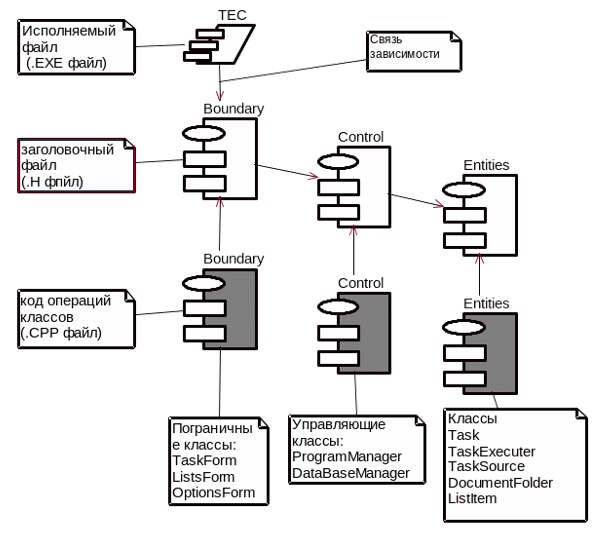
\includegraphics[width=1\linewidth]{Img 2}}
\caption{Диаграмма компонентов}
\label{comp:image}
\end{figure}

Веб-страница передает данные компоненту в момент вызова последнего. На рисунке 3.2 показана схема компонентов при вызове компонента на странице сайта.

\begin{figure}[H]
\center{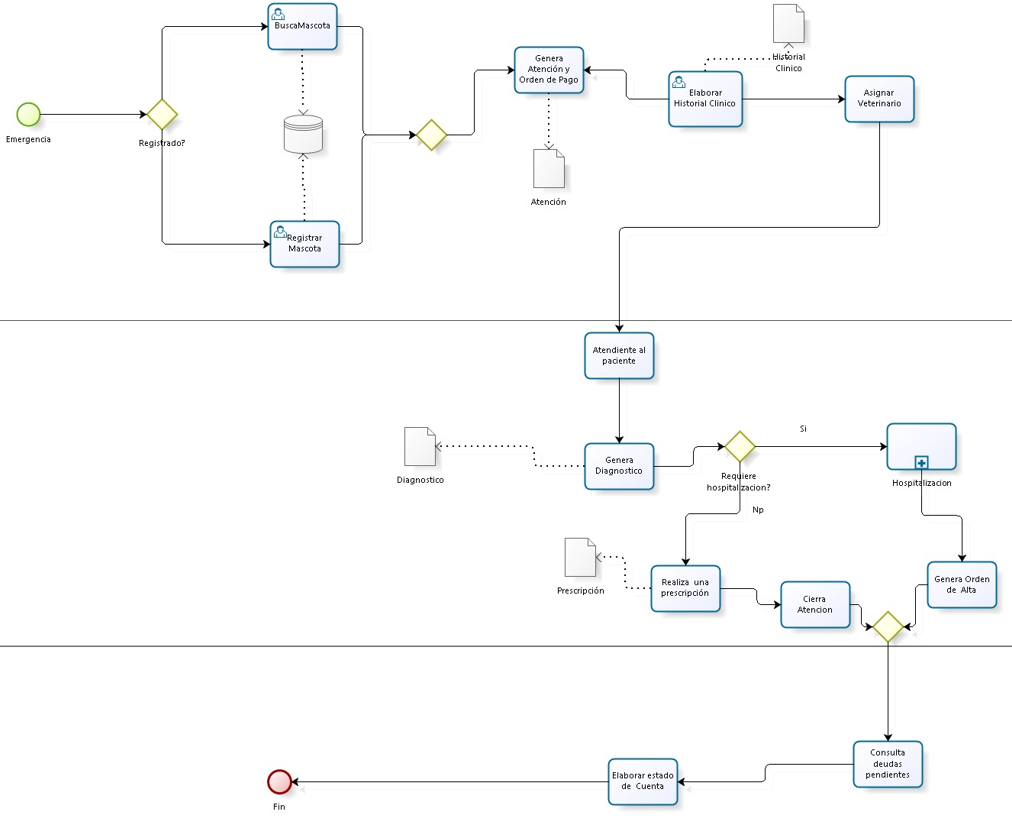
\includegraphics[width=1\linewidth]{Img 3}}
\caption{Диаграмма компонентов}
\label{data:image}
\end{figure}

\subsection{Диаграмма размещения}

Диаграмма размещения (рис.~\ref{place:image}) отражает физические взаимосвязи между программными и аппаратными компонентами системы. Она является хорошим средством для показа маршрутов перемещения объектов и компонентов в распределенной системе.

\subsection{Диаграмма таблицы MySQL}
Диаграммы таблиц в MySQL — полезный инструмент для визуализации структуры базы данных и отношений между ее таблицами, поскольку они облегчают понимание структуры базы данных.

Таблицы подобны контейнерам для базы данных, чтобы разделить ее на более мелкие части, чтобы хранить информацию в отдельном и более организованном виде.

Когда дело доходит до хранения данных в базе данных, вы можете использовать несколько различных подходов.

MySQL использует подход, называемый реляционной базой данных.

В реляционной базе данных ваши данные разбиваются на несколько отдельных областей хранения, называемых таблицами, вместо того, чтобы объединять все в одну большую единицу хранения.

Для решения этих проблем реляционная база данных будет использовать отдельную таблицу для клиентов и отдельную таблицу для заказов.

Используя нечто, называемое «ключом», вы сможете связать данные, вы увидите, что использует эта реляционная модель, при этом все ваши данные будут разделены на отдельные таблицы.

В MySQL вы можете создать несколько баз данных и внутри них вы можете создать несколько таблиц. В свою очередь, эти таблицы могут содержать множество данных, которые можно создавать, удалять, изменять или просматривать различными способами.

используя график таблицы могут просто и наглядно представлять структуру базы данных MySQL и помощь в ее создании, имея глобальное видение структуры базы данных,
его легче правильно спроектировать и создать.
Диаграмма на рис. 3.4 показывает мертвые таблицы, созданные с помощью с помощью MySQL.

\begin{figure}[H]
	\center{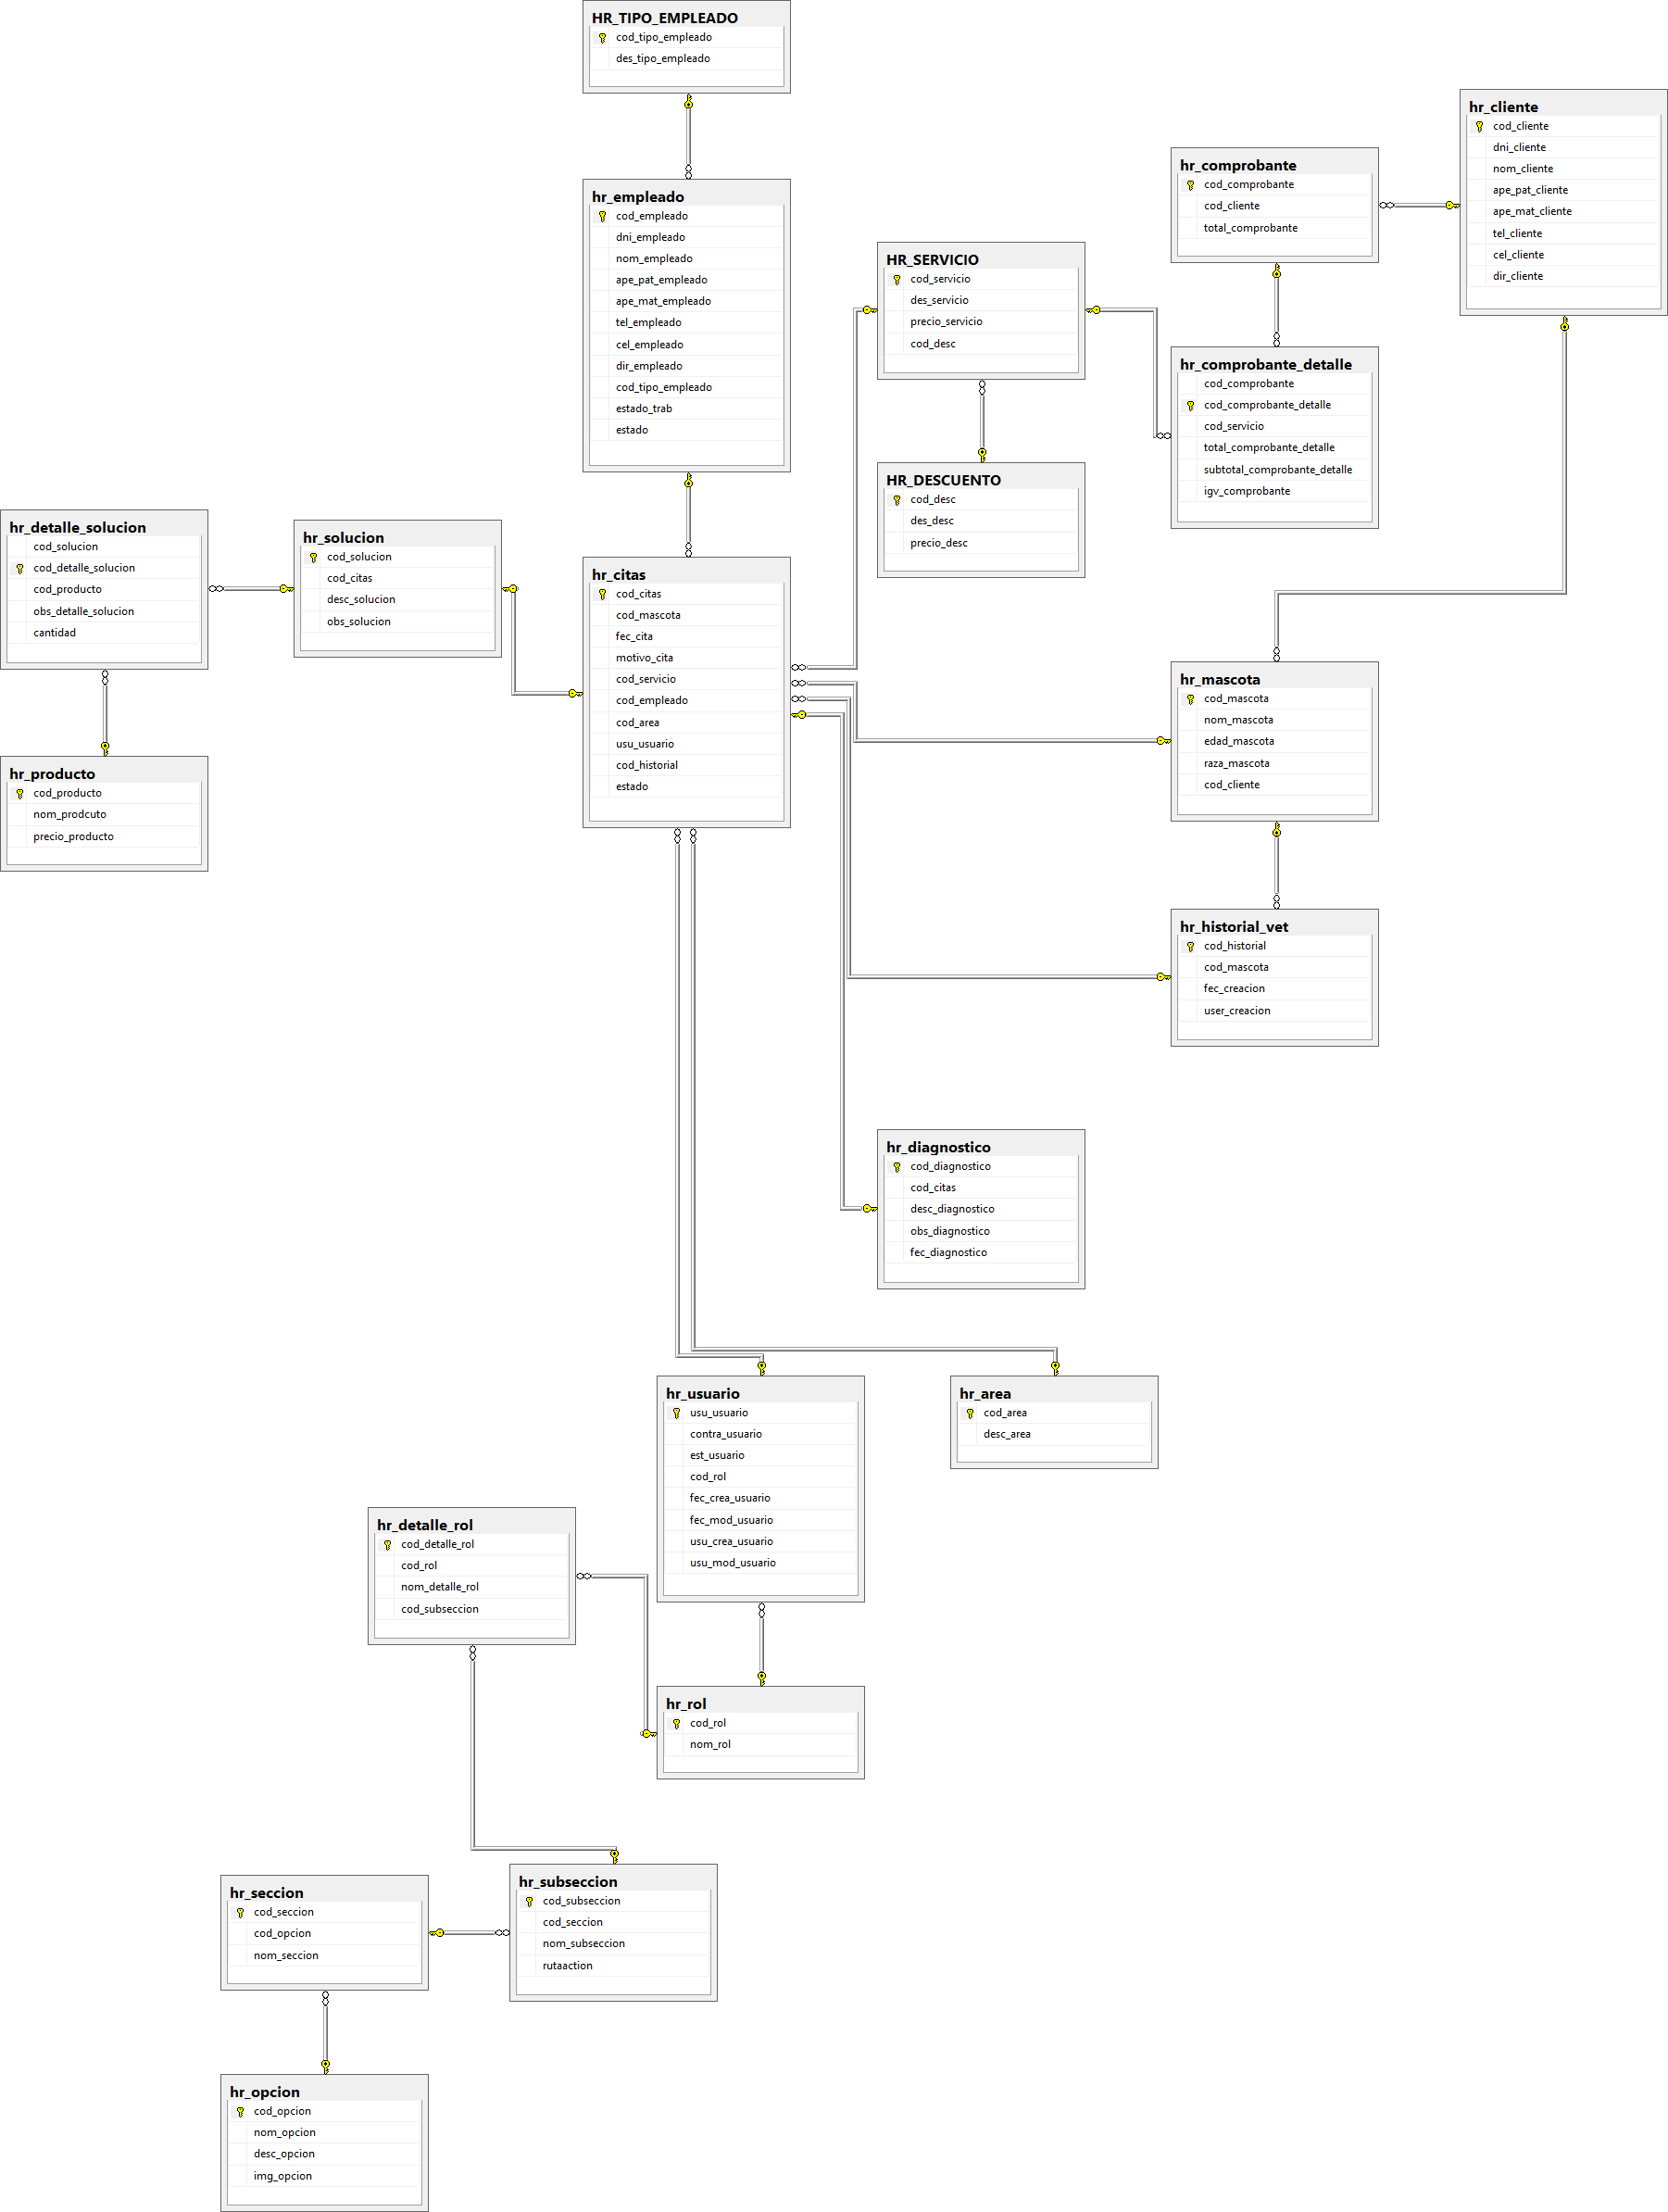
\includegraphics[width=1\linewidth]{Img 9}}
	\caption{Диаграмма на мертвые таблицы}
	\label{data:image}
\end{figure}


\subsection{Содержание информационных блоков. Основные сущности}

Проанализировав требования, можно выделить шесть основных сущностей:
\begin{itemize}
\item ``Empleado'' - В таблице «Empleado» находится испанский перевод слова врачу, относящегося к врачу.;
\item ``Cliente'' - В таблице «Сliente» приведен испанский перевод слова клиента, относящегося к владельцам животных.
\item ``Mascota'' - В таблице «Mascota» приведен испанский перевод слова животных, относящийся к животным..
\end{itemize}

В состав сущности ``empleado'' можно включить атрибуты, представленные в таблице.

\begin{longtable}[l]{|C{7.5cm}|C{3.5cm}|C{3.5cm}|}
\caption{Атрибуты сущности ``Empleado''\label{news:table}}\\
\hline Поле & Тип & Обязательное \\
\hline 1 & 2 & 3 \\
\endfirsthead
\caption*{Продолжение таблицы \ref{news:table}}\\
\hline 1 & 2 & 3 \\
\endhead
  \hline ID & string & true \\
  \hline cod\_empleado & int & true \\
  \hline dni\_empleado & int & true \\
  \hline ape\_pat\_empleado & varchar & true \\
  \hline ape\_mat\_empleado & varchar & true \\
  \hline tel\_empleado & int & true \\
  \hline cel\_empleado & int & true \\
  \hline dir\_empleado & varchar & true \\
  \hline cod\_tipo\_empleado & int & true \\
  \hline estado\_tipo & varchar & true \\
  \hline estado & varchar & true \\
  \hline
\end{longtable}

В состав сущности “врачу” включить атрибуты, представленные в
таблице 3.1.

\begin{longtable}[l]{|C{7.5cm}|C{3.5cm}|C{3.5cm}|}
	\caption{Атрибуты сущности ``cliente''\label{news:table}}\\
	\hline Поле & Тип & Обязательное \\
	\hline 1 & 2 & 3 \\
	\endfirsthead
	\caption*{Продолжение таблицы \ref{news:table}}\\
	\hline 1 & 2 & 3 \\
	\endhead
	\hline ID & string & true \\
	\hline cod\_cliente & int & true \\
	\hline dni\_cliente & int & true \\
	\hline nom\_cliente & varchar & true \\
	\hline ape\_pat\_cliente & varchar & true \\
	\hline ape\_mat\_cliente & varchar & true \\
	\hline tel\_cliente & int & true \\
	\hline cel\_cliente & int & true \\
	\hline dir\_cliente & varchar & true \\
	\hline
\end{longtable}

В состав сущности “клиента” включить атрибуты, представленные в
таблице 3.2.

\begin{longtable}[l]{|C{7.5cm}|C{3.5cm}|C{3.5cm}|}
	\caption{Атрибуты сущности ``Mascota''\label{news:table}}\\
	\hline Поле & Тип & Обязательное \\
	\hline 1 & 2 & 3 \\
	\endfirsthead
	\caption*{Продолжение таблицы \ref{news:table}}\\
	\hline 1 & 2 & 3 \\
	\endhead
	\hline ID & string & true \\
	\hline cod\_mascota & int & true \\
	\hline nom\_mascota & varchar & true \\
	\hline edad\_mascota & varchar & true \\
	\hline raza\_mascota & varchar & true \\
	\hline cod\_cliente & int & true \\
	\hline
\end{longtable}

В состав сущности “животных” включить атрибуты, представленные в
таблице 3.3.


Система имеет интегрированный механизм, соединяющий различные
разделы и элементы информационных блоков, что означает отсутствие необходимости добавления дополнительных идентификаторов для связи между
различными сущностями.

Информационные блоки содержат элементы, которые представляют
сущности, а эти элементы, в свою очередь, имеют поля и свойства, которые
представляют атрибуты этих сущностей. Таким образом, нет необходимости
добавлять дополнительные идентификаторы для связи между различными
частями системы.

В системе предусмотрен внутренний механизм связи между разделами и элементами информационных блоков, поэтому введения дополнительных идентификаторов при реализации связей между сущностями не предполагается.

Экземпляры сущностей реализуются в информационных блоках посредством элементов, атрибуты сущности – посредством полей и свойств элемента. 
